\documentclass{article}

% if you need to pass options to natbib, use, e.g.:
% \PassOptionsToPackage{numbers, compress}{natbib}
% before loading nips_2018

\usepackage[preprint]{nips_2018}
% to compile a preprint version, e.g., for submission to arXiv, add
% add the [preprint] option:
% \usepackage[preprint]{nips_2018}

% to compile a camera-ready version, add the [final] option, e.g.:
% \usepackage[final]{nips_2018}

% to avoid loading the natbib package, add option nonatbib:
% \usepackage[nonatbib]{nips_2018}

\usepackage[utf8]{inputenc} % allow utf-8 input
\usepackage[T1]{fontenc}    % use 8-bit T1 fonts
\usepackage{hyperref}       % hyperlinks
\usepackage{url}            % simple URL typesetting
\usepackage{booktabs}       % professional-quality tables
\usepackage{amsfonts}       % blackboard math symbols
\usepackage{nicefrac}       % compact symbols for 1/2, etc.
\usepackage{microtype}      % microtypography
\usepackage{amsmath}
\usepackage{algorithm}
\usepackage{algorithmicx}
\usepackage{algpseudocode}
% \usepackage{palatino}
\usepackage{tikz}
\usetikzlibrary{shapes.geometric, arrows}
\title{A Brief Report of Deep Ritz Method}

% The \author macro works with any number of authors. There are two
% commands used to separate the names and addresses of multiple
% authors: \And and \AND.
%
% Using \And between authors leaves it to LaTeX to determine where to
% break the lines. Using \AND forces a line break at that point. So,
% if LaTeX puts 3 of 4 authors names on the first line, and the last
% on the second line, try using \AND instead of \And before the third
% author name.

\author{
  Zeyu Jia\\School of Mathematical Science\\Peking University\\ \texttt{1600010603} \\
  \And
  Dinghuai Zhang\\School of Mathematical Science\\Peking University\\ \texttt{1600013525}\\
  \And
  Zhengming Zou\\School of Mathematical Science\\Peking University \\ \texttt{1600011089}
}

\begin{document}
% \nipsfinalcopy is no longer used

\maketitle

\begin{abstract}
\par For long people have met great difficulties when solving numerical partial differential equations (PDEs), especially in high-dimensional conditions. In order to solve partial differential equations effectively, Yu and E proposed the deep Ritz method \cite{yu2017deep}, combining the traditional Ritz method with deep learning. With residual blocks and stochastic gradient descent, it works well under both low-dimensional and high-dimensional conditions. In this report we delve deeper into their work and propose several improvements on their models, includeing the self-adaptive regularization and actor-critic self-adaptive method. Besides, we also do numerical experiments by ourselves, and our improvements make the deep Ritz method work better. 
\end{abstract}

\section{Introduction}
\par Partial differential equation \cite{evans1998partial} is an important tool to characterize our world mathematically. From physics to chemistry, and from financial to engineering, partial differential equations always play an indispensable role. However, partial differential equation is always very hard to solve, and at most of the time it is impossible. So in practice, we often find some ways to simplify the original partial differential equations, and solve them. To achieve this goal, we also need to figure out some ways to solve these simplified partial differential equations, or at least, find their approximate solutions.
\par The simplified partial differential equation we are going to discuss in this report is the Poisson equation 
\eqref{poisson}
\begin{equation}\label{poisson}
	\begin{cases}
		\Delta u = f, \qquad\forall x\in\Omega,\\
		u = g, \qquad\forall x\in\partial\Omega.
	\end{cases}
\end{equation}
\par The traditional partial differential equation solving methods include finite difference method \cite{strikwerda2004finite}, finite volume method \cite{versteeg2007introduction} and finite element method \cite{brenner2007mathematical}. These methods are the most commonly used. And complete theories for these methods, such as consistency, stability and convergence, have been well established. However, these methods will become tough, even impossible, to complicated functions or high dimension situation. Even though the convergence still holds, the time complexity it guarantees will not permit such enormous calculations. Thus, we need to develop some methods to tackle these difficulties.
\par Deep learning \cite{lecun2015deep} has been well developed recently. Benefited from its well approximating ability, flexibility and power to tackle the curse of dimensionality, we have achieved state of arts on so many missions, such as classification, object detection and so on. So it is natural to think about a suitable way to use deep learning to solve partial differential equations. \cite{yu2017deep} proposed a method to approximate the solution by a neural network, and use the well-known Ritz method to solve the variational problem. \cite{1707.02568}\cite{weinan2017deep}\cite{beck2017machine} first transfer partial differential equations into backward stochastic differential equations, and then use neural networks or other machine learning methods to approximate their solutions.
\par In this report, what we focus on is Deep Ritz Method \cite{yu2017deep}. We derive the theory of this algorithm, give our own interpretations and propose several novel ideas to this algorithm, including the self-adaptive sampling method and actor-critic self-adaptive sampling method. The self-adaptive sampling method, which samples points for regularization based on the approximate error, aims to improve the efficiency of the algorithm by sampling more points where functions are not fitted well and sampling less points where functions are fitted well. And the actor-critic self-adaptive sampling method is proposed to find a better function of approximation errors into sampling distribution. We also write our own numerical experiments and make some comparison between the original methods and methods we proposed.
\par The plan of this report is as follows: In section 2, we will give a brief introduction to Ritz method, which is the basis of deep Ritz method. The structure of deep Ritz method will be shown in section 3. In section 4, our novelty to the deep Ritz method will be exhibited and illustrated. And finally in section 5, we will present the numerical experiments we have done by ourselves and their interpretation.

\section{The Ritz Method}  % 这里我觉得需要一个Ritz Method的引用,Evans或者贾泽宇发的那本数值pde都可以
\par The Ritz method \cite{evans1998partial} is a method based on the principle of least action to find the approximation to eigenvalue equations that cannot be solved easily (or at all) analytically. Mathematically, the Ritz method can be used to approximate the solution of partial differential equations in a function space. When we aim to seek a function $y(x)$ that maximize or minimize an integral $I(y(x))$. Suppose that we can approximate $y(x)$ with a linear combination of some linear independent functions:
\begin{equation}
	y(x)=\varphi_0(x)+k_1\varphi_1(x)+...+\varphi_N(x).
\end{equation}
Where $\varphi_{i}(x),i\in\{1,2,...,N\}$ are a basis of the function space we are interested in. In many cases, we use the basis 
\begin{equation}
	\begin{aligned}
		\cos x, \cos 2x, \cdots, \cos nx, \cdots\\
		\sin x, \sin 2x, \cdots, \sin nx, \cdots
	\end{aligned}
\end{equation}
However, this basis is of infinite dimension, which means it is very tough to solve. So we always restrict our solutions space in finite dimension.
\par Next we take the homogeneous Dirichlet boundary value problem of the Poisson equation \eqref{possion_equation} as an example.
\begin{equation}\label{possion_equation}
	\begin{cases}
 		\Delta u=-f(x), & x\in \Omega, \\
 		u=0, & x\in \partial \Omega. \\
 	\end{cases}
\end{equation}
The weak solution of \eqref{possion_equation} corresponding to the principle of least action is
\begin{equation}\label{variational problem}
	\begin{cases}
 		\text{Find }\ u\in H_{0}(\Omega),\quad s.t.\\
 		I(u)=\min\limits_{v\in H_{0}(\Omega)} I(v),\\
  	\end{cases}
\end{equation}
where $H_{0}(\Omega)$ is the set of admissible functions. Using variational method, we can prove that 
\begin{equation}\label{functional_I}
I(v)=\int_\Omega\left(\frac{1}{2}|\nabla v(x)|^2-f(x)v(x)\right)dx. 
\end{equation}
As a matter of fact, if we assume that $v$ is an n-dimensional function, then
\begin{equation}\label{d_I}
\delta I(v)=\int _{\Omega} \left(\frac{\partial v}{\partial x_1}\cdot \delta \frac{\partial v}{\partial x_1}+...+\frac{\partial v}{\partial x_n}\cdot   \delta \frac{\partial v}{\partial x_n}-f(x)\delta      v(x)   \right)dx.
\end{equation}
Using the integration by parts method for several integrals,
\begin{equation}\label{int_by_parts}
\int _{\Omega}\frac{\partial v}{\partial x_i}\cdot \delta \frac{\partial v}{\partial x_i} dx= \frac{\partial v}{\partial x_i}\cdot \delta v\Big|_{\partial \Omega}-\int_{\Omega}\delta v \cdot \frac{\partial^2 v}{\partial x_i ^2}dx=-\int_{\Omega}\delta v \cdot \frac{\partial^2 v}{\partial x_i ^2}. \qquad 1\le i\le n
\end{equation}
Substituting \eqref{int_by_parts} into \eqref{d_I} we can obtain the following equation.
\begin{equation}
\delta I(v)=-\int_{\Omega}\delta v(\Delta v+f(x))dx=0
\end{equation}
\par Because of the strongly convexity of the functional $I$ in \eqref{functional_I}, the solution of \eqref{variational problem} is unique. Hence the solution of \eqref{variational problem} is identical to \eqref{possion_equation}.

\section{Deep Ritz Method with neural networks}
\par Using the Ritz Method mentioned above, it is natural to think of solving partial differential equations with deep neural networks. Considering the partial differential equation
\begin{equation}
\Delta u(x)+f(x)=0,\qquad x\in \Omega.
\end {equation}
\par According to Ritz Method, what we need to do is
\begin{equation}\label{optimization problem}
\min\limits_{u\in H}{I(u)},
\end{equation}
where
\begin{equation}\label{I_equ}
I(u)=\int_\Omega\left(\frac{1}{2}|\nabla u(x)|^2-f(x)u(x)\right)dx,
\end{equation}
and $H$ is the set of admissible function. Our main idea is to facilitate the multi-layer neural network approximation function $u(x)$ and use the stochastic gradient descent algorithm to solve the optimization problem \eqref{optimization problem}.

\subsection{Building Trail Function}
\par We use a nonlinear transformation $x \to u_{\theta}(x)$ defined by deep neural networks to approximate function $u(x)$. Here $\theta$ denotes network parameters in our model. Similar to ResNet structure, we use several blocks to construct our networks, where each block consists of two linear transformations, two activation functions and one residual connection. The $i$-th block can be expressed as 
\begin{equation}\label{res_equ}
	s_i=\phi(W_{i2}\cdot\phi(W_{i1}\cdot s_{i_1}+b_{i1})+b_{i2})+s_{i-1},
\end{equation}

where $s_{i}$ is the output of the $i$-th layer, $W_{i1},W_{i2}\in R^{m\times m},b_{i1},b_{i2}\in R^{m}$ and $\phi$ is the activation function.

\begin{figure}
	\centering
	\setlength{\belowcaptionskip}{10pt}
	\caption{Network Structure of Deep Ritz Method}
	\label{architecture}
	\tikzstyle{startstop} = [rectangle, rounded corners, minimum width = 2cm, minimum height=1cm,text centered, draw = black, fill=red]
	\tikzstyle{io} = [trapezium, trapezium left angle=80, rounded corners = 2mm, trapezium right angle=100, minimum width=2cm, minimum height=1cm, text centered, draw=black, fill=purple!50]
	\tikzstyle{process} = [rectangle, rounded corners = 2mm, minimum width=3cm, minimum height=0.5cm, text centered, draw=black, fill=pink!50]
	\tikzstyle{decision} = [diamond, aspect = 3, text centered, draw=black, fill=blue!30, align = center]
	\tikzstyle{add} = [rectangle, minimum size=6mm, rounded corners=3mm, very thick, draw=black!50, top color=white, bottom color=black!20]
	% 箭头形式
	\tikzstyle{arrow} = [->,>=stealth]
	\begin{tikzpicture}[node distance = 1cm]
	%定义流程图具体形状
	\node[io,  yshift = -1cm](in1){Input};
	\node(fc11) [process, below of = in1, yshift = -0.3cm]{FC layer(size m)};
	\node(fc12) [process, below of = fc11]{Activate};
	\node(add1) [add, below of = fc12]{+};
	\node(fc21) [process, below of = add1]{FC layer(size m)};
	\node(fc22) [process, below of = fc21]{Activate};
	\node(add2) [add, below of = fc22]{+};
	\node(fc31) [process, below of = add2]{FC layer(size m)};
	\node(fc32) [process, below of = fc31]{Activate};
	\node(add3) [add, below of = fc32]{+};
	\node(residual 1) [decision, right of = fc11, xshift = 5cm, yshift= -0.5cm]{Residue\\Connection};
	\node(residual 2) [decision, right of = fc21, xshift = 5cm, yshift= -0.5cm]{Residue\\Connection};
	\node(residual 3) [decision, right of = fc31, xshift = 5cm, yshift= -0.5cm]{Residue\\Connection};
	\node(fc4) [process, below of = add3]{FC layer(size 1) };
	\node(out1) [io, below of = fc4, yshift = -0.3cm]{Output};
	%连接具体形状
	\draw [arrow] (in1) -- (fc11);
	\draw [arrow] (0, -1.8) -| node  [right] {} (residual 1);
	\draw [arrow] (fc11) -- (fc12);
	\draw [arrow] (fc12) -- (add1);
	\draw [arrow] (residual 1) |- node [right] {} (add1);
	\draw [arrow] (add1) -- (fc21);
	\draw [arrow] (0, -4.8) -| node  [right] {} (residual 2);
	\draw [arrow] (fc21) -- (fc22);
	\draw [arrow] (fc22) -- (add2);
	\draw [arrow] (residual 2) |- node [right] {} (add2);
	\draw [arrow] (add2) -- (fc31);
	\draw [arrow] (0, -7.8) -| node  [right] {} (residual 3);
	\draw [arrow] (fc31) -- (fc32);
	\draw [arrow] (fc32) -- (add3);
	\draw [arrow] (residual 3) |- node [right] {} (add3);
	\draw [arrow] (add3) -- (fc4);
	\draw [arrow] (fc4) -- (out1);
	\end{tikzpicture}
\end{figure}

\par Because our partial differential equation involves the Laplacian transform, we hope that the second derivative of the function $u(x)$ is not a constant. To ensure the smoothness of function $u_{\theta}$, we apply the non-linear function \eqref{non linear} as the activation function, instead of ReLU (rectified linear unit) function.
\begin{equation}\label{non linear}
	\phi(x)=\max\{x^3,0\}. 
\end{equation}

\par The residual connection in \cite{he2016deep} helps to avoid gradient vanishing problems. After several blocks, we adopt a linear transform to the final result. The architecture of residual connection can be viewed in \ref{architecture}. And the whole network can be expressed as
\begin{equation}
	u_{\theta}(x)=a\cdot f_n(x) \circ ...\circ f_1(x)+b,
\end{equation}
where $f_i(x)$ is the $i$-th block and $a\in R^m, b\in R$. Note that the input vector $x$ is not necessarily $m$-dimensional. In order to handle this mismatch, we can pad $x$ with a vector of zeros. In our model, we always assume $d<m$.
\par After building our trail functions, the rest of our work is to minimize the $I(u)$ in (\ref{I_equ})

\subsection{Euler Numerical Integration Method}   
\par The first problem we need to deal with is to calculate the integral in (\ref{I_equ})
 . For simplicity, we define:
 \begin{equation}
 g(x,\theta)=|\nabla u(x)|^2-f(x)u(x)
 \end{equation}
 then $I(u)$ can be expressed as
 \begin{equation}
 I(u)=\int _{\Omega}g(x,\theta)dx
 \end{equation}
 Obviously, it's impossible to calculate this integral directly. We use Euler integration method to approximate the integral.
 \begin{equation}
 I(u)=L(x,\theta)=\frac{1}{N}\sum\limits_{i=1}^{N}g(x_i,\theta),
 \end{equation}
 where $x_i$ is taken from the uniform grid on the domain with steps 0.001.
 \subsection{The Stochastic Gradient Descent Algorithm}
 During the training process of neural networks, stochastic gradient descent (SGD) is a commonly used method for optimization. In this problem, we also choose stochastic gradient descent method to minimize $I(u)$. This optimization process can be expressed as:
 \begin{equation}
 \theta^{k+1}=\theta^{k}-\eta \nabla_{\theta}\frac{1}{N}\sum\limits_{i=1}^{N}g(x_{i,k},\theta^k),
 \end{equation}
 where $\{x_{i,k}\}$ is the randomly selected from uniform grid points. In our settings, we use mini-batch stochastic gradient descent algorithm and Adam \cite{kingma2014adam} optimizer to optimize.

\section{Our Improvements}
\par Along with the footsteps of professor E, we have achieved very good results. Based on the results already available, we want to make further improvements. 


\subsection{Self-Adaptive Sampling}
\par In order to find out the tougher place and enhance the regularization, we use a self-adaptive sampling method here. This idea is similar to adaptive finite element method in chapter 9 of \cite{brenner2007mathematical}, which refines the grid adaptively according to the difficulty of each grid. (this difficulty is described by the value of $f$ given the PDE $\Delta u = f$.) 
\par Here we adopt the self adaptive method on the regularization terms, which are the boundary constraints or interior constraints. Suppose the neural network function is $f(x) = \mathrm{NN}(x, \theta_k)$, then we will use the following adaptive method to sample:
\begin{itemize}
	\item For the boundary restrictions, we sample points according to density function $|f(x)|$ where $x$ is on the boundary of $\partial\Omega$.
	\item For interior, we sample uniformly for the variation, and sample according to density function $|\Delta(x) - f(x)|$.
\end{itemize}
\par  According to this method, more points will be sampled at places where the neural network does not fit well, and less points will be sampled at places where the neural network fits well. 

\subsection{Actor-Critic Self-Adaptive Sampling}
\par From the numerical experiments of self-adaptive sampling method, we find out that the self-adaptive method works better. However, there is one problem still involved in. That is, we actually do not know which distribution of sampling is the most suitable way, and can achieve the best regularization effect. In the discussion of the last subsection, we choose the distribution to be proportional to the error between $\Delta(x)$ and $f(x)$. This choice seems plausible, but we cannot make sure that the error we choose in this way is perfect. Hence we introduce the following actor-critic way to sampling. And for simplicity, we only discussed about the self-adaptive sampling method on the boundary (the situation in the interior is similar to this).
\par Actor-critic \cite{konda2000actor} is a famous method in reinforcement learning. The core idea is similar to generative adversarial networks (GAN) \cite{goodfellow2014generative}, both of which design two networks, an actor (generative) network and a critic (discriminator) network. The task of the actor is to generate a distribution or a policy, and the task of the critic is to analyze the difference between the generated distribution and the real distribution.
\par In our settings, we use the actor to generate a distribution which can be used for sampling points for regularization, as we discussed above. Some assumptions need to be clarified first. That is, we assume the density function of the distribution is a function of the error \eqref{error} (In the last subsection, the density function is identity to the the error). 
\begin{equation}\label{error}
	\pi(x) = \phi(err(x), \theta_{a}),
\end{equation}
where $err(x)$ is the error function at $x$, $\theta_{a}$ is the parameter of network, and $\pi(x)$ is the desirable sampling distribution. Besides, we also assume that the function $\phi$ only depends on the domain $\Omega$ and has nothing to do with the partial differential equation. Hence the actor is a network which takes the approximate error as input and output the sampling distribution. And in \eqref{error} it is the function $\phi$ with network parameters $\theta_{a}$. 
\par As for critic network in our settings, distinguished from \cite{goodfellow2014generative} \cite{konda2000actor}, we use the critic network to test the effectiveness of the sampling distribution generated by the actor. This network $\psi(u_{approx}, u_{real}, \theta_{c})$ will give and effective measure of error between the approximate solution and the real solution. We assume that the network parameters only depend on $\Omega$ as well, like the actor network.
\par As for the training for both neural network, based on the assumption that only the shape of domain could influence $\theta_{a}, \theta_{c}$. Given the domain $\Omega$, we first choose some rather simple functions. Then we initialize solutions for their corresponding Poisson equations (do not need to be accurate) and apply deep Ritz method to solve for a few iterations. Besides, we also adopt some numerical methods, such as finite difference method or finite element method. And compare the solutions of these numerical methods and deep Ritz method by our critic network to give the loss. Then we can train the actor network to minimize the losses and train the critic network to maximize the losses. The whole process can be viewed in algorithm 
\ref{ac-algorithm} and figure \ref{ac-figure}
\begin{algorithm}
	\caption{Actor-critic Self-adaptive Training}
	\label{ac-algorithm}
	\begin{algorithmic}[1]
		\State\textbf{Input} Domain $\Omega$, $m, t$.
		\State Generate some rather simple functions $f_1, f_{2}, \cdots, f_{m}$ defined on $\Omega$.
		\State Solve these partial differential equations finite difference method or finite element method with different grid sizes. And obtain approximate solutions $v_{1}^{j}, \cdots, v_{m}^{j}, 1\le j\le t$
		\State For each $1\le i\le m$, find $t$ initial solutions $u_{i}^{1}, \cdots, u_{i}^{t}$ randomly.
		\State Use the current actor network parameter $\theta_{a}$ to generate sampling distributions for $u_{i}^{1}, \cdots, u_{i}^{t}$.
		\State Train the original network with these distribution to obtain $u_{i}'^{1}, \cdots, u_{i}'^{t}$.
		\State Put $u_{i}'^{j}$ and $v_{i}^{j}$ into the critic network with parameter $\theta_{c}$, and obtain the loss $\mathcal{L}_{i}^{j}$.
		\State Train $\theta_{a}$ to minimize the sum of loss $\mathcal{L}_{i}^{j}$.
		\State Train $\theta_{c}$ to maximize the sum of loss $\mathcal{L}_{i}^{j}$.
 	\end{algorithmic}
\end{algorithm}

\begin{figure}
    \centering
    \setlength{\belowcaptionskip}{10pt}
    \caption{Architecture of Algorithm}
    \label{ac-figure}
    \tikzstyle{rec} = [rectangle, rounded corners=2mm, fill = yellow!50, minimum width = 2cm, minimum height = 1cm, text centered, draw = black, align=center]
    \tikzstyle{rec1} = [rectangle, rounded corners=2mm, fill = red!50, minimum width = 2cm, minimum height = 1cm, text centered, draw = black, align=center]
    \tikzstyle{rec2} = [rectangle, rounded corners=2mm, fill = blue!50, minimum width = 2cm, minimum height = 1cm, text centered, draw = black, align=center]
    \tikzstyle{arrow} = [thick, ->, draw = blue]
    \tikzstyle{arrow1} = [thick, ->, draw = red]
    \tikzstyle{line} = [thick, -, draw = blue]
    \begin{tikzpicture}[node distance = 1cm]
    	\node(origin)[rec]{Original\\network $f$};
        \node(error)[rec1, right of = origin, xshift = 2cm]{Error};
        \node(actor)[rec, below of = error, yshift = -3cm]{Actor $\phi_{a}$};
		\node(distribution)[rec2, below of = origin, yshift = -1cm]{Distribution $\pi$};
		\node(decreasing)[rec1, left of = origin, xshift = -2cm]{Decreasing $\Delta l$};
		\node(critic)[rec, below of = decreasing, yshift = -1cm]{Critic $\phi_{c}$};
		\node(critic_loss)[rec1, below of = critic, yshift = -1cm]{Loss $\mathcal{L}$};
		\node(train_critic) at (-5.8, -3) {Critic Training};
        \draw[arrow] (origin) -- (error);
        \draw[arrow] (distribution) -- (origin) node[midway, right] {Sampling};
        \draw[line] (error) -- (3, -2);
        \draw[line] (actor) -- (3, -2);
        \draw[arrow] (3, -2) -- (distribution);
        \draw[arrow] (origin) -- (decreasing);
        \draw[arrow] (decreasing) -- (critic);
        \draw[arrow] (distribution) -- (critic);
        \draw[arrow] (critic) -- (critic_loss);
        \draw[arrow1] (critic_loss) to [out=180, in=180] (critic);
        \draw[arrow1] (critic_loss) -- (actor) node[midway, below] {Actor Training};
    \end{tikzpicture}
\end{figure}

\section{Numerical Results}

\subsection{The Poisson Equation}
\par Considering the Poisson equation:
\begin{equation}
\left\{
\begin{aligned}
 \Delta u=1,& x\in \Omega \\
 u=0, &x\in \partial \Omega \\
 \end{aligned}
\right.
\end{equation}

Here $\Omega =\{(x,y)| x^2+y^2<1\}$.
\par The exact solution to this problem is 
\begin{equation}
u=\frac{1}{4}(x^2+y^2-1)
\end{equation}

\par As described above, we use three blocks (six fully connected layers) and a final linear transform with $m=10$ to build our networks. There is a total of 671 parameters in our model. Considering the boundary condition, we need to make some modifications to our model. We have decided to use a penalty method and the modified function is:
\begin{equation}\label{functional}
I(u)=\int_{\Omega}\left(\frac{1}{2}|\nabla u(x)|^2-u(x)\right)dx+\gamma\int_{\Omega}|\Delta u(x) - 1|^2dx+\beta\int_{\partial \Omega}u(x)^2dx
\end{equation}
Where $\gamma\int_{\Omega}|\Delta u(x) - 1|^2dx$ is the regular term and $\beta\int_{\partial \Omega}u(x)^2dx$ is the penalty item.We choose $\beta=500$ and $\gamma=500$.
\par After 400 iterations, the relative loss of our model is reduced to $1.3\%$. Our training results of Deep Ritz Method is shown in Figure \ref{3.1a}

\begin{figure}[ht]
 	 \centering
 	 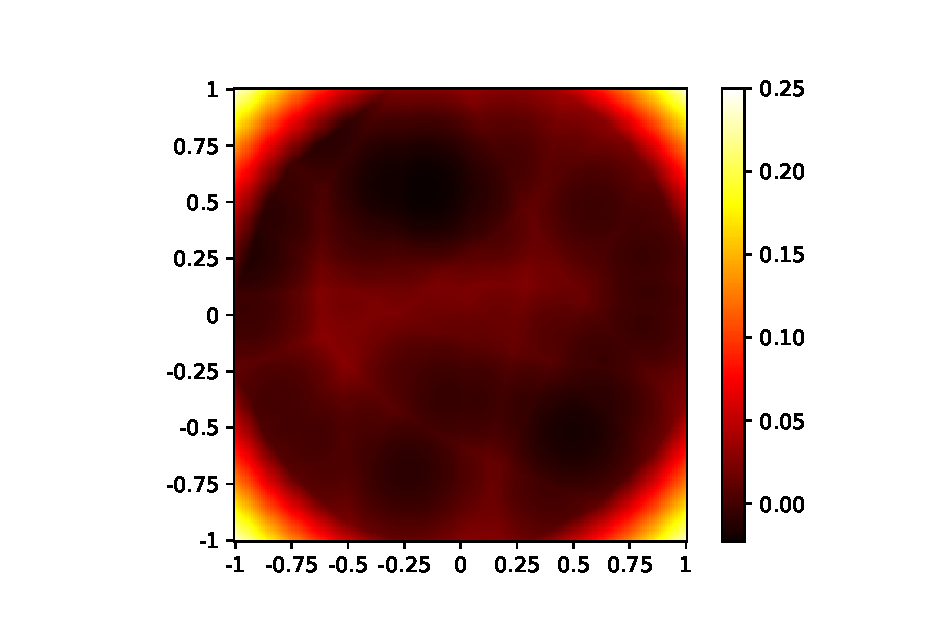
\includegraphics[width=0.6\textwidth]{./images/loss_3-1.eps} 
	 \caption {The results of Poisson Equation}
	 \label{3.1a}
\end{figure}
As is shown from the figure, the dark color indicates that the absolute error between the numerical solution and the real solution is small, while the light color indicates that the absolute error between the numerical solution and the real solution is relatively large.Deep Ritz method performs well with this problem after 400 iterations.

\par After testing models of different layers, we find that the 3-layers model with 671 parameters performed best on this problem. Our numerical results of relative error computed by $l_2$-norm is shown in Table \ref{different layers of poisson equation}. Too many parameters may lead overfitting, limiting the performance of the networks.

\begin{table}[htbp]
\centering  
\caption{Relative loss of different layers with Poisson Eqaution}
\label{different layers of poisson equation}
\begin{tabular}{ccc} 
	\toprule  %添加表格头部粗线
	Blocks Num & Parameters & Relative Loss (\%) \\
	\hline
	1 & 231 & 3.2\\
	\hline
	2 & 451 & 2.0\\
	\hline
	3 & 671 & 1.3\\
	\hline
	4 & 891 & 1.5\\
	\bottomrule %添加表格底部粗线
\end{tabular}
\end{table}

\subsection{The Poisson Equation in High Dimension}
As for high dimension equation, our model can also do well. Considering Poisson Equation in higher dimension:

\begin{equation}
\left \{
\begin{aligned}
&-\Delta u =0, &x\in (0,1)^{10} \\
&u(x)=\sum_{k=1}^5x_{2k-1}x_{2k}, &x\in \partial (0,1)^{10}
\end{aligned}
\right.
\end{equation}

The exact solution for this equation is 
\begin{equation}
u(x)=\sum\limits_{k=1}^5x_{2k-1}x_{2k}.
\end{equation}
The network we used this time has the same structure as \ref{poisson_in_2d}. We still use three blocks (six fully connected layers) and a final linear transform with m = 10 to build our networks. But there are some differences in the penalty items. This time we let the learning rate increase with the number of iterations, which can lead to a better training results. The learning rate can be expressed as:
\begin{equation}
\beta=\beta_{0}^N
\end{equation}
Where $N$ is the number of iteration. We choose $\beta_0=1.01$.

\subsection{Other Poisson Equation}
\par Considering the following Poisson Equation:
\begin{equation}
\left\{
\begin{aligned}
& \Delta u=0, & x\in \Omega \\
 &u=xy,   &x\in \partial \Omega \\
 \end{aligned}
\right.
\end{equation}

Here $\Omega =\{(x,y)| 0<x,y<1\}$.
\par The exact solution to this problem is 
\begin{equation}
u=xy
\end{equation}
Compared with the equation in \ref{functional}, there are some differences in the penalty items. This time we let the learning rate increase with the number of iterations, which can lead to a better training results. The learning rate can be expressed as:
\begin{equation}
\beta=\beta_{0}^N
\end{equation}
Where $N$ is the number of iteration.After a few attempts, we choose $\beta_0=1.01$. After 5000 iterations, the relative loss of our model is reduced to 1.4\%. Our training result is shown in Figure \ref{3.2a}
\begin{figure}[ht]
 	 \centering
 	 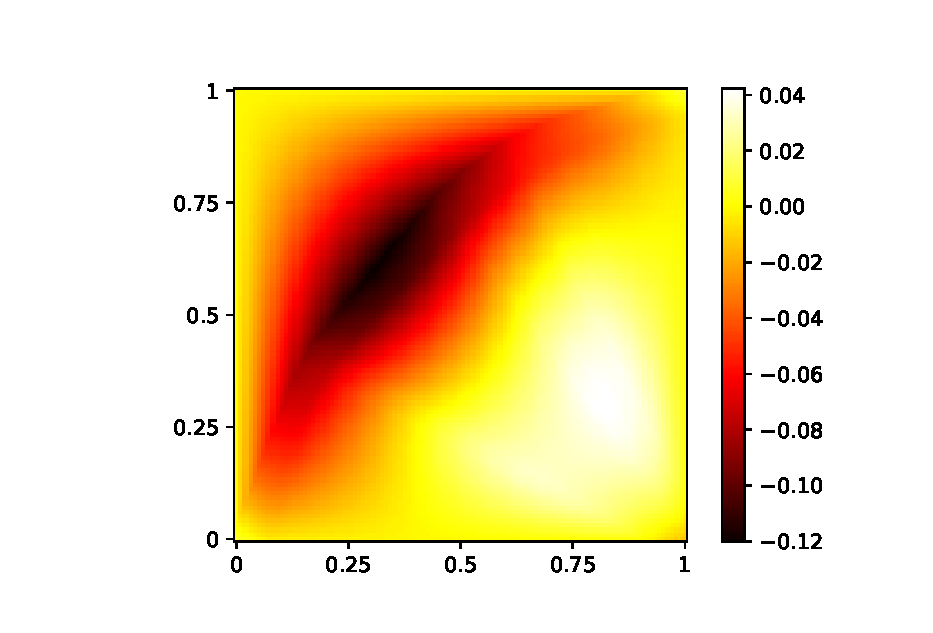
\includegraphics[width=0.6\textwidth]{./images/loss_yubing.eps} 
	 \caption {The results of Poisson Equation}
	 \label{3.2a}
\end{figure}

Same as before, the color depth in the graph reflects the absolute error from the exact value.

\section{Conclusion and Discussions}

In this project report, we demonstrate that our method is simple but effective when solving a certain series of PDEs. What's more, we can achieve higher accuracy with proper improvement as follows:

\begin{enumerate}
\item
%I don't know how to descibe (\delta u - f) !!
Add a regularization term to punish the norm of lapacian operator. 
\item
Adjust loss coeffecients according to it's shift from  extreme value. We call it \emph{adaptive} method.
\item
Introduce reinforcement learning to adjust the adaptive coeffecients.
\end{enumerate}

While having achieved fairish results, there exist many drawbacks and probable amelioration which we will handle in the future work:

%maybe more ``future work'' can be added here.
\begin{enumerate}
\item
Our method is not robust enough for general application. Sometimes much tuning work is needed for a single PDE.
\item

\item

\end{enumerate}

\section*{Acknowledgement}
%Thanks luyiping

\bibliography{reference}
\bibliographystyle{plain}


\medskip

\small

\end{document}
